\section{非线性演化方程的三种波解}
\begin{frame}
\frametitle{非线性演化方程的三种波解}
\begin{enumerate}
\item \Painleve{}展开法得到变换.
\item 简单 Hirota 方法得到孤子解.
\item 共轭参数法得到呼吸子解.
\item 长极限法得到 lump 解.
\end{enumerate}
\end{frame}

\subsection{\Painleve{}展开法}
\begin{frame}
\frametitle{\Painleve{}展开法}
\begin{columns}
\small 
\begin{column}{0.5\textwidth}
理论:
\[
    u=u(x_1,\cdots,x_n,t)
\]
\[
    U(u,u\up{1},u\up{2},u\up{3}\cdots)=0
\]
\[
    u=\sum_{k=1}^m{\frac{u_k}{f^{m-k+1}}}=\frac{u_1}{f^m}+\cdots+\frac{u_m}{f}
\]
\[
    F(f,f\up{1},f\up{2},f\up{3}\cdots)=0
\]
改进:
\begin{itemize}
\item TPE 是对数变换的推广.
\item $m$ 通过$n$阶展开方法确定, 能比齐次平衡原则得到更多的解.
\item 对 $u_k$ 的求解提出了递归算法, 更加全面地考虑了可能出现的情况.
\end{itemize}
\end{column}
\begin{column}{0.5\textwidth}
例子: (3+1) Jimbo-Miwa 方程
\[
    u_{xxxy}+3u_{xx}u_y+3u_{x}u_{xy}+2u_{ty}-3u_{xz}=0
\]
\[
    u=\frac{2f_x}{f}=2\sbrace{\ln f}_x
\]
\[
\begin{split}
    0&=2\,{f}^{2}f_{{{ txy}}}+{f}^{2}f_{{{ xxxxy}}}-3\,{f}^{2}f_{{{ xxz}}}\\
    &-2\,ff_{{t}}f_{{{ xy}}}-2\,ff_{{{ tx}}}f_{{y}}-2\,ff_{{{ ty}}}f_{{x}}\\
    &-4\,ff_{{x}}f_{{{ xxxy}}}+6\,ff_{{x}}f_{{{ xz}}}+3\,ff_{{{ xx}}}f_{{z}}\\
    &+2\,ff_{{{ xxx}}}f_{{{xy}}}-ff_{{{ xxxx}}}f_{{y}}\\
    &+4\,f_{{t}}f_{{x}}f_{{y}}+6\,{f_{{x}}}^{2}f_{{{ xxy}}}-6\,{f_{{x}}}^{2}f_{{z}}\\
    &-6\,f_{{x}}f_{{{ xx}}}f_{{{ xy}}}+2\,f_{{x}}f_{{{ xxx}}}f_{{y}}
\end{split}
\]
\end{column}
\end{columns}
\end{frame}

\subsection{Hirota 方法与孤子解}
\begin{frame}
\frametitle{Hirota 方法与孤子解}
\begin{columns}
\small 
\begin{column}{0.5\textwidth}
行波变换:
\[
\begin{split}
    \xi&=p_1\sbrace{x_1+p_2x_2+\cdots+p_nx_n+\omega t} \\ 
    &+p_{n+1}
\end{split}
\]
\[
    \PS\subseteq  \ALLP=\bbrace{1,2,\cdots,n,n+1}
\]
\[
    S(e,k;\PS): \left\{\begin{array}{ll}
        p_i \rightarrow p_{i,k} & i \in \PS, \\ 
        p_i \rightarrow p_i & i \not\in \PS.
    \end{array}\right.
\]
\[
    \xi_i=S(xi,i,\PS)
\]
\end{column}
\begin{column}{0.5\textwidth}
例子:
\[
    \xi=k(x+py+qz+\omega t)+c
\]
\[
    \PS=\bbrace{1,2}
\]
\[
\begin{split}
    \xi_i&=k_i\sbrace{x+p_iy+qz+\frac{3q-k_i^2p_i}{2p_i}t}+c, \\ 
    \xi_j&=k_j\sbrace{x+p_jy+qz+\frac{3q-k_j^2p_j}{2p_j}t}+c.
\end{split} 
\]
\end{column}
\end{columns}
\end{frame}

\begin{frame}
孤子解公式:
\[
\begin{split}
    f_{m-soliton}&=\sum_{\mu=0,1}\exp\sbrace{\sum_{i=1}^m{\mu_i \xi_i}+\sum_{1\le i<j\le m}{\mu_i\mu_jH_{i,j}}} \\ 
    &=\sum_{P\subseteq M}\mbrace{\sbrace{\prod_{\bbrace{i,j}\subseteq P}{h_{i,j}}}\exp\sbrace{\sum_{k\in P}{\xi_k}}}
\end{split}
\]
\[
    M=\bbrace{1,2,\cdots,m},~~\xi_k=S(\xi,k;\PS)
\]
例子:
\[
\begin{split}
    f_1&=1+\exp\sbrace{\xi_1} \\ 
    f_2&=1+\exp\sbrace{\xi_1}+\exp\sbrace{\xi_2}+h_{1,2}\exp\sbrace{\xi_1+\xi_2} \\ 
    f_3&=1+\exp(\xi_1)+\exp(\xi_2)+\exp(\xi_3)\\
       &+h_{1,2}\exp(\xi_1+\xi_2)+h_{2,3}\exp(\xi_2+\xi_3)+h_{1,3}\exp(\xi_1+\xi_3)\\
       &+h_{1,2}h_{2,3}h_{1,3}\exp(\xi_1+\xi_2+\xi_3)
\end{split}
\]
\end{frame}

\begin{frame} 
\[
\begin{split}
    F(f_1)=0 &\Rightarrow \omega \\ 
    F(f_2)=0 &\Rightarrow h_{i,j} 
\end{split}
\]
\[
\begin{split}
    \omega &= \frac{3q-k^2p}{2p} \\ 
    h_{i,j}&=\frac{(k_ip_j(k_i-k_j)+q)p_i^2-p_ip_j(k_jp_j(k_i-k_j)+2q)+qp_j^2}{(k_ip_j(k_i+k_j)+q)p_i^2+p_ip_j(k_jp_j(k_i+k_j)-2q)+qp_j^2}
\end{split}
\]
\begin{figure}
\centering 
\subfigure[1-孤子解 \label{jm:1-soliton}]{
    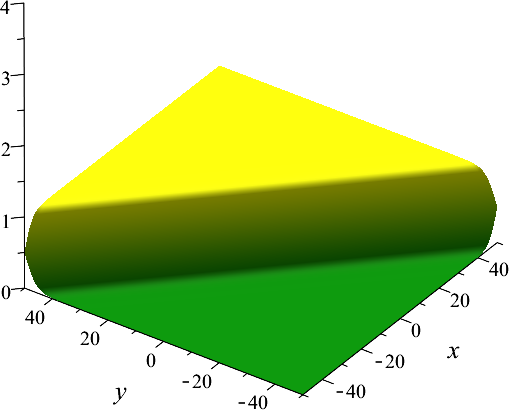
\includegraphics[width=.3\textwidth]{../paper/fig/(3+1)JM-1-soliton.png}    
}
\subfigure[2-孤子解 \label{jm:2-soliton}]{
    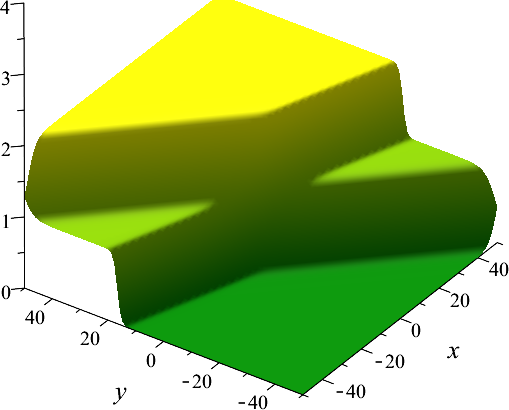
\includegraphics[width=.3\textwidth]{../paper/fig/(3+1)JM-2-soliton.png}
}
\subfigure[3-孤子解 \label{jm:3-soliton}]{
    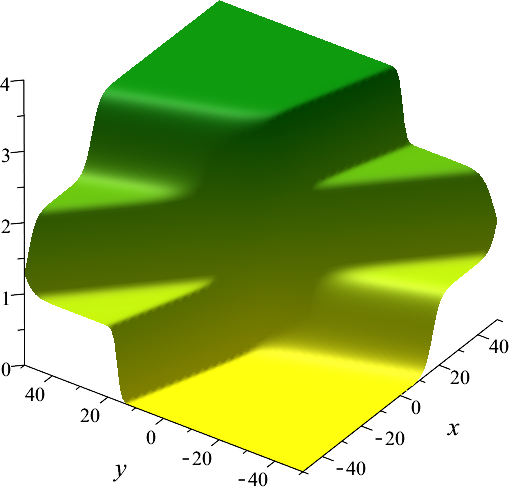
\includegraphics[width=.3\textwidth]{../paper/fig/(3+1)JM-3-soliton.png}
}
\end{figure}
\end{frame}

\subsection{共轭参数法与呼吸子解}
\begin{frame}
\frametitle{共轭参数法与呼吸子解}
\begin{columns}
\begin{column}{0.5\textwidth}
理论:
\[
    f_{m-breather}=\conj{f_{(2m)-soliton}} 
\]
\[
    p_{i,j}=p_{i,j+m}^*,~(j=1,2,\cdots,m)
\]
\[
\begin{split}
    p_{i,j}&=p_{i,j,RE}+I\cdot p_{i,j,IM}, \\ 
    p_{i,j+m}&=p_{i,j,RE}-I\cdot p_{i,j,IM},
\end{split}
\]
\end{column}
\begin{column}{0.5\textwidth}
例子: $m=1,\PS=\bbrace{1,2}$,\\$\xi=k(x+py+qz+\omega t)+c$.
\[
\begin{split}
    k_1&=k_{1,RE}+I\cdot k_{1,IM} \\ 
    k_2&=k_{1,RE}-I\cdot k_{1,IM} \\
    p_1&=p_{1,RE}-I\cdot p_{1,IM} \\
    p_2&=p_{1,RE}+I\cdot p_{1,IM} \\ 
\end{split} 
\]
\end{column}
\end{columns}
\end{frame}

\begin{frame}
\begin{figure}
\setcounter{subfigure}{0}
\subfigure[1-呼吸子解 \label{jm:1-breather}]{
    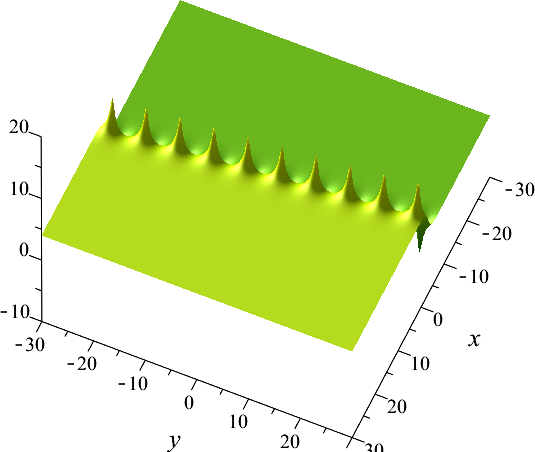
\includegraphics[width=.3\textwidth]{../paper/fig/(3+1)JM-1-breather.png}
}
\subfigure[2-呼吸子解 \label{jm:2-breather}]{
    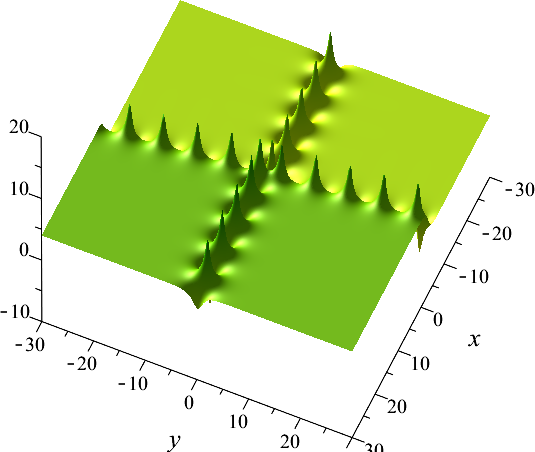
\includegraphics[width=.3\textwidth]{../paper/fig/(3+1)JM-2-breather.png}
}
\subfigure[3-呼吸子解 \label{jm:3-breather}]{
    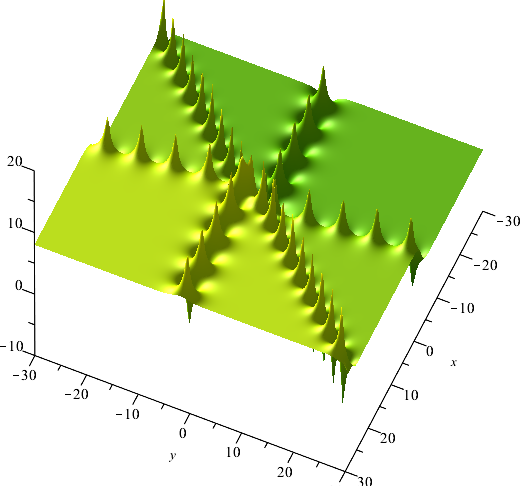
\includegraphics[width=.3\textwidth]{../paper/fig/(3+1)JM-3-breather.png}
}
\subfigure[周期波解 \label{jm:1-periodic}]{
    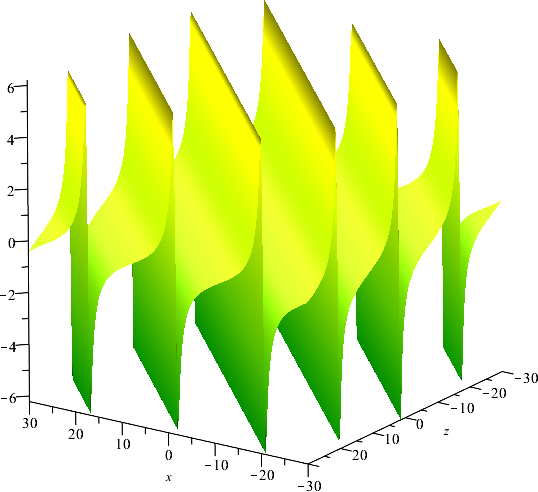
\includegraphics[width=.3\textwidth]{../paper/fig/(3+1)JM-1-periodic.png}
}
\subfigure[孤子-呼吸子相互作用解 \label{jm:soliton-breather}]{
    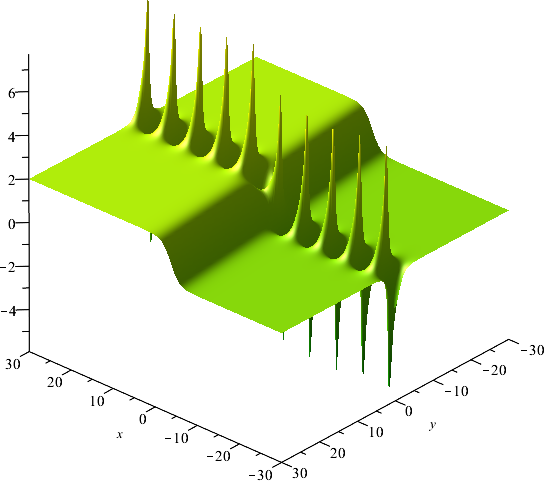
\includegraphics[width=.3\textwidth]{../paper/fig/(3+1)JM-soliton-breather.png}
}
\end{figure}
\end{frame}

\subsection{长极限法与 lump 解}
\begin{frame}
\frametitle{长极限法与 lump 解}
生成公式:
\[
    f_{m-lump}=\conj{\Theta_m}
\]
\[
\begin{split}
    \Theta_m&=\prod_{k=1}^{2m}\theta_k+\frac{1}{2}\sum_{i,j}{b_{i,j}}\prod_{J\neq i,j}{\theta_J}+\frac{1}{2! 2^2}\sum_{i,j,k,l}{b_{i,j}b_{k,l}}\prod_{J\neq i,j,k,l}{\theta_{J}}+\cdots \\
    &+\frac{1}{s!2^s}\sum_{i,j,\cdots,u,v}\underbrace{{b_{i,j}b_{k,l}\cdots b_{u,v}}}_{s}\prod_{J\neq i,j,\cdots, u,v}{\theta_J}+\cdots 
\end{split}
\]
例子:
\[
\begin{split}
\Theta_1&=\theta_{1}\theta_{2}+b_{12} \\
\Theta_2&=\theta_{1}\theta_{2}\theta_{3}\theta_{4}+b_{12}\theta_{3}\theta_{4}+b_{13}\theta_{2}\theta_{4}+b_{14}\theta_{2}\theta_{3}+b_{23}\theta_{1}\theta_{4}\\
&+b_{24}\theta_{1}\theta_{3}+b_{34}\theta_{1}\theta_{2}+b_{12}b_{34}+b_{13}b_{34}+b_{14}b_{23}
\end{split}
\]
\end{frame}

\begin{frame}
重写生成公式
\[
    f_{m-lump}=\sum_{l=0}^m\sum_{s\in L(l)}\sbrace{\prod_{k=1}^l{b_{s_{2k-1},s_{2k}}}\prod_{p\not\in s}{\theta_p}}
\]
\[
    L(l)=\bbrace{\sbrace{s_1, s_2, \cdots ,s_{2l}}\left|s_{2k}>s_{2k-1},s_{2k+1}>s_{2k-1},s_k\in \bbrace{1,\cdots,2l}\right.}
\]
\begin{itemize}
\item $s_{2k}>s_{2k-1}$ 保证了$b_{i,j}=b_{j,i}$的等价情况只出现一次. 
\item $s_{2k+1}>s_{2k-1}$ 保证了$b_{i,j}$的全排列只出现一次.
\end{itemize}
\end{frame}

\begin{frame}
\begin{columns}
\begin{column}{0.5\textwidth}
关键参数:
\[
\begin{split}
    \theta &= \eval{\frac{\partial \xi}{\partial p_1}}{p_1=0}, \\
    b_{i,j}&= \eval{\frac{\partial^2}{\partial p_{1,i}\partial p_{1,j}}h_{i,j}}{p_{1,i}=0,p_{1,j}=0}.
\end{split}
\]
\end{column}
\begin{column}{0.5\textwidth}
例子:
\[
\begin{split}
    &\theta=\frac{2p^2y+(2qz+2x)p+3qt}{2p}, \\ 
    &b_{i,j}=-\frac{2p_ip_j(p_i+p_j)}{q(p_i-p_j)^2}.
\end{split}
\]
\end{column}
\end{columns}
\begin{figure}
\setcounter{subfigure}{0}
\centering 
\subfigure[1-lump解 \label{jm:1-lump}]{
    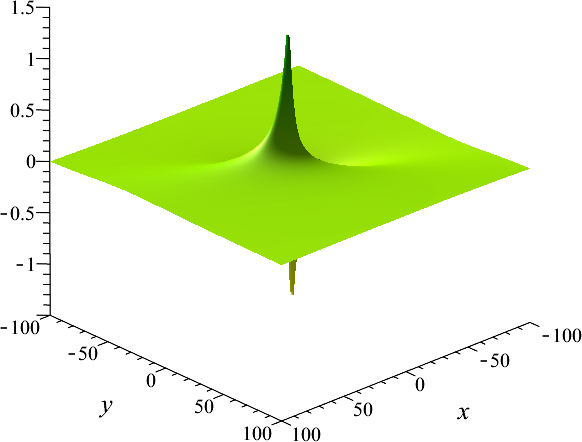
\includegraphics[width=.3\textwidth]{../paper/fig/(3+1)JM-1-lump.png}
}
\subfigure[2-lump解 \label{jm:2-lump}]{
    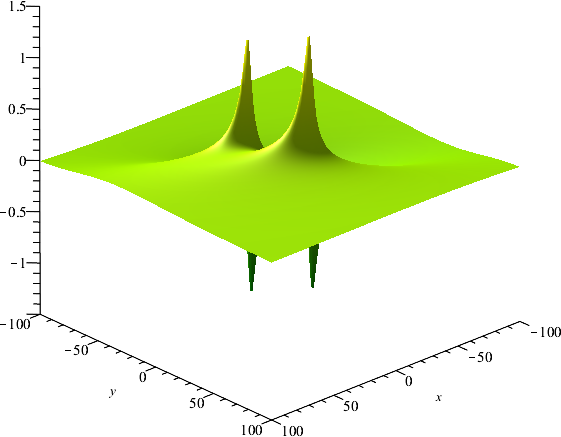
\includegraphics[width=.3\textwidth]{../paper/fig/(3+1)JM-2-lump.png}
}
\subfigure[3-lump解 \label{jm:3-lump}]{
    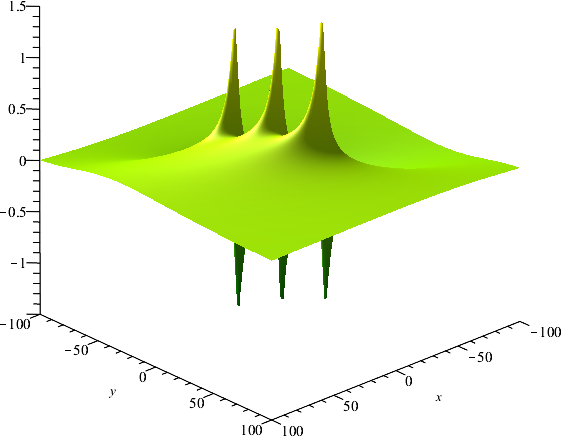
\includegraphics[width=.3\textwidth]{../paper/fig/(3+1)JM-3-lump.png}
}
\end{figure}
\end{frame}

\subsection{实验与分析}
\begin{frame}
\frametitle{实验与分析}
\begin{columns}
\begin{column}{0.65\textwidth}
\begin{table}
\centering
\small 
\begin{tabular}{lcccc}
\hline
\multicolumn{1}{c}{方程名} & 1 & 12 & 13 & 123 \\ 
\hline
(1+1)KdV & \tpa\tpb & & & \\
(2+1)BKP-T & \tpa\tpb & \tpa\tpa & & \\
(2+1)KP &\tpa\tpb &\tpa\tpa & & \\
(2+1)SK &\tpa\tpb &\tpa\tpa & & \\
(4+1)Fokas-T-2 &\tpa\tpb &\tpa\tpa & & \\
(2+1)CBS & \tpa\tpb & \tpa\tpb & & \\
(2+1)CBS-G & \tpa\tpb & \tpc\tpc & & \\
(3+1)CBS &\tpa\tpb &\tpa\tpb &\tpa\tpb &\tpa\tpb \\
(3+1)BKP &\tpa\tpb &\tpa\tpa &\tpa\tpa &\tpc\tpc \\
(3+1)KP &\tpa\tpb &\tpa\tpa &\tpa\tpa &\tpc\tpc \\
(3+1)JM &\tpa\tpb &\tpa\tpa &\tpa\tpb &\tpc\tpc \\
(3+1)NEE-T &\tpa\tpb &\tpa\tpa &\tpa\tpb &\tpc\tpc \\
(3+1)YTSF &\tpa\tpb &\tpa\tpa &\tpa\tpb &\tpb\,\tpb \\
(4+1)Fokas-T &\tpa\tpb &\tpa\tpb &\tpa\tpb &\tpc\tpc \\
\hline
\end{tabular}
\end{table}
\end{column}
\begin{column}{0.35\textwidth}
\begin{itemize}
\item `\tpa{}' 表示能够满足原方程.
\item `\tpb{}' 表示有解不能得到解.
\item `\tpc{}' 表示有解但不满足原方程.
\item 第一个对应3孤子解, 第二个对应2 lump解.
\end{itemize}
\end{column}
\end{columns}
\end{frame}